\chapter{Esperimenti}
\section{Exp-1}
\section{Exp-2}
\section{Exp-3}
\section{Exp-4}
\section{Exp-5}

\section{Valutazioni Test-Set}
\textcolor{red}{INSERIRE intro sul fatto che abbiamo valutato singoli char e frasi}:

\subsection{Singoli caratteri}
La valutazione sui singoli caratteri si articola in due diverse analisi:
\begin{itemize}
    \item Curve Precision-Recall
    \item Matrice di confusione
\end{itemize}

\subsubsection*{Curve Precision-Recall}
Le curve Precision-Recall (PR) consentono di analizzare il bilanciamento tra \emph{precision} e \emph{recall} nelle predizioni del modello, mostrando quanto esso riesca a mantenere alta la precisione man mano che aumenta la quantità di caratteri correttamente riconosciuti. Un indicatore sintetico della qualità complessiva è l'area sotto la curva (AUC-PR), che risulta tanto più elevata quanto migliore è la capacità del modello di conciliare accuratezza e sensibilità nel riconoscimento dei caratteri.

\subsubsection*{Risultati}
In Figura~\ref{fig:pr_curves} sono riportate le curve per un sottoinsieme rappresentativo di classi non confondibili.

\textcolor{red}{INSERIRE quelle nuove}:
\begin{figure}[htbp]
    \centering
    \begin{subfigure}[t]{0.32\textwidth}
        \centering
        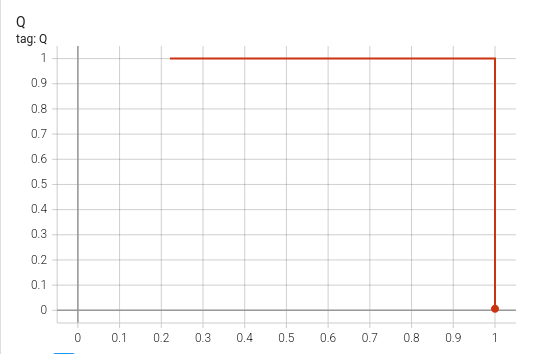
\includegraphics[width=\textwidth]{images/pr_curve1.png}
        \caption{PR-curve \{'\}}
    \end{subfigure}
    \begin{subfigure}[t]{0.32\textwidth}
        \centering
        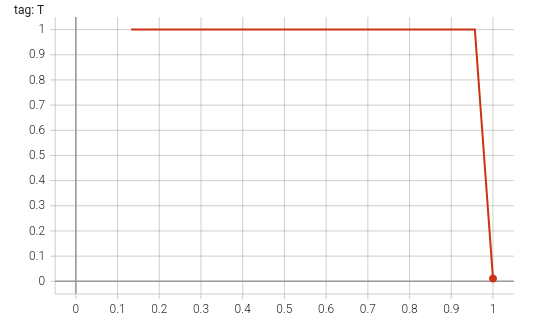
\includegraphics[width=\textwidth]{images/pr_curve2.png}
        \caption{PR-curve \{T\}}
    \end{subfigure}
    \begin{subfigure}[t]{0.32\textwidth}
        \centering
        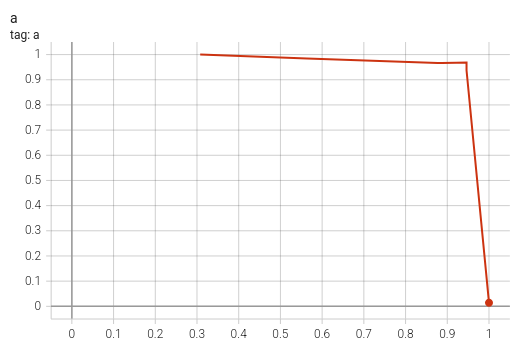
\includegraphics[width=\textwidth]{images/pr_curve3.png}
        \caption{PR-curve \{Y\}}
    \end{subfigure}
    \caption{PR-curves per caratteri non confondibili}
    \label{fig:pr_curves}
\end{figure}

Nel complesso, il modello mostra buone prestazioni, con curve PR ampie e stabili per la maggior parte delle classi.

Tuttavia, alcune classi risultano più problematiche. Come visibile in Figura~\ref{fig:pr-confondibili}.

\textcolor{red}{INSERIRE quelle nuove}:
\begin{figure}[htbp]
    \centering
    \begin{subfigure}[t]{0.32\textwidth}
        \centering
        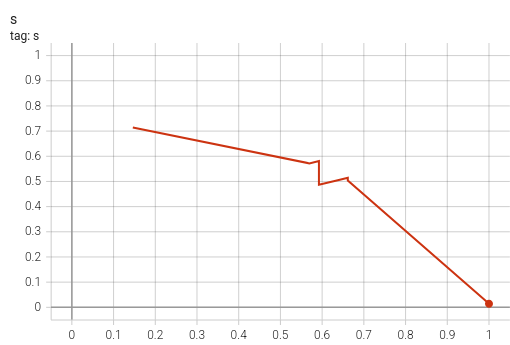
\includegraphics[width=\textwidth]{images/pr_curve_conf1.png}
        \caption{PR-curve \{s\}}
    \end{subfigure}
    \begin{subfigure}[t]{0.32\textwidth}
        \centering
        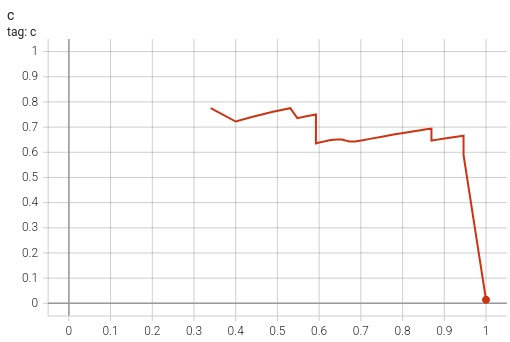
\includegraphics[width=\textwidth]{images/pr_curve_conf2.png}
        \caption{PR-curve \{c\}}
    \end{subfigure}
    \begin{subfigure}[t]{0.32\textwidth}
        \centering
        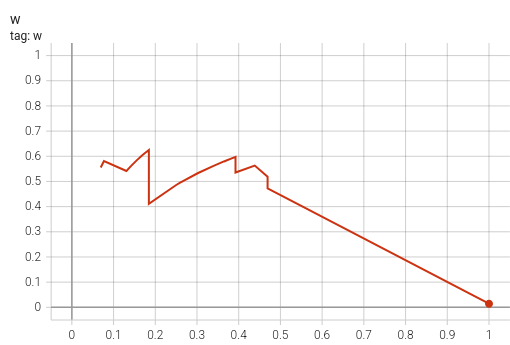
\includegraphics[width=\textwidth]{images/pr_curve_conf3.png}
        \caption{PR-curve \{v\}}
    \end{subfigure}
    \caption{PR-curves per caratteri confondibili}
    \label{fig:pr-confondibili}
\end{figure}

Per valutare l'impatto della distinzione tra maiuscole e minuscole, è stata ripetuta l'analisi ignorando il case. Come mostrato in Figura~\ref{fig:pr-ignore}, l'area sotto la curva migliora sensibilmente, suggerendo che una parte consistente degli errori è dovuta a una difficoltà del modello nel distinguere il case piuttosto che a un'incapacità di riconoscere la forma del carattere.
\textcolor{red}{INSERIRE quelle nuove}:
\begin{figure}[htbp]
    \centering
    \begin{subfigure}[t]{0.32\textwidth}
        \centering
        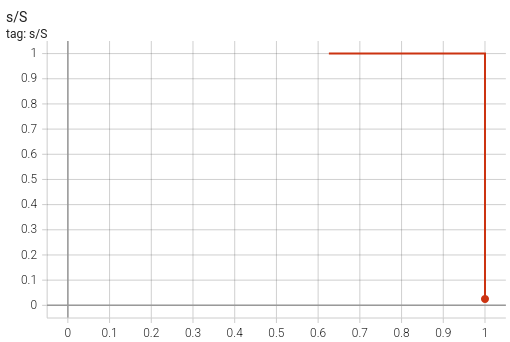
\includegraphics[width=\textwidth]{images/pr_ignore1.png}
        \caption{PR-curve \{s/S\}}
    \end{subfigure}
    \begin{subfigure}[t]{0.32\textwidth}
        \centering
        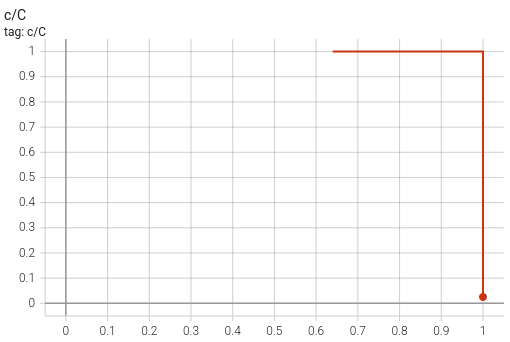
\includegraphics[width=\textwidth]{images/pr_ignore2.png}
        \caption{PR-curve \{c/C\}}
    \end{subfigure}
    \begin{subfigure}[t]{0.32\textwidth}
        \centering
        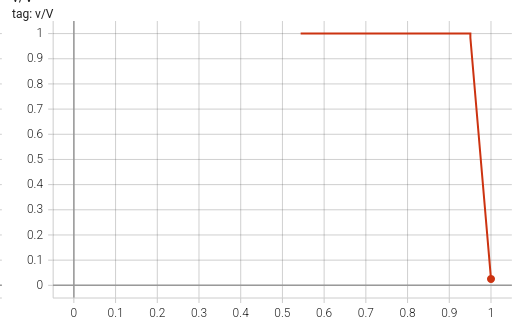
\includegraphics[width=\textwidth]{images/pr_ignore3.png}
        \caption{PR-curve \{v/V\}}
    \end{subfigure}
    \caption{PR-curves ignorando il case}
    \label{fig:pr-ignore}
\end{figure}

Questi risultati suggeriscono che, pur in presenza di buone prestazioni globali, il modello potrebbe beneficiare delle euristiche di post-processing.


\subsection{Matrice di confusione}
\textcolor{red}{INSERIRE i vari case riportati su sheet}

La matrice di confusione aggregata a livello di carattere, mostrata in Figura~\ref{fig:confusion_matrix}, offre una panoramica dettagliata sugli errori di classificazione del modello. Ogni cella \((i, j)\) della matrice rappresenta il numero di volte in cui un carattere \(i\) è stato classificato dal modello come appartenente alla classe \(j\).

\begin{figure}[htbp]
    \centering
    \includegraphics[width=0.65\textwidth]{images/confusion_matrix.png}
    \caption{Matrice di confusione}
    \label{fig:confusion_matrix}
\end{figure}

Si osserva come la diagonale principale della matrice sia in gran parte ben marcata, indicando una prevalenza di classificazioni corrette. Le deviazioni più evidenti dalla diagonale si concentrano invece in corrispondenza di coppie di caratteri visivamente simili, che il modello tende a confondere con maggiore frequenza.

Questa osservazione conferma la precedente analisi delle PR-curves: la maggior parte degli errori è riconducibile a un numero limitato di classi particolarmente confondibili.

Nel repository del progetto è disponibile una matrice di confusione completa sotto forma di report HTML.

\subsection{Valutazione parole}
\label{sec:valutazione-stringhe}

Per l'analisi a livello di parola sono state adottate due metriche principali:
\begin{enumerate}
    \item Distanza di edit (\emph{Levenshtein distance \footnote{V. I. Levenshtein, “Binary codes capable of correcting deletions, insertions and reversals,” \textit{Soviet Physics Doklady}, vol. 10, pp. 707-710, 1966.} });
    \item String Accuracy.
\end{enumerate}

I calcoli sono stati effettuati sui dataset degli screenshot descritti nella \autoref{sec:dataset_screenshots}, che comprendono due tipologie di dati:
\begin{itemize}
    \item sequenze di 10 simboli casuali;
    \item frasi di senso compiuto.
\end{itemize}

\subsection{Distanza di edit}

La distanza di edit tra la parola riconosciuta e la parola ground-truth è stata calcolata per ciascun esempio, normalizzando il valore sulla lunghezza della parola.

Di seguito si riporta una tabella con le statistiche principali (media, mediana e deviazione standard) della distanza di edit normalizzata, calcolate separatamente per i due dataset.

\textcolor{red}{INSERIRE valori reali dopo fix errori}

\begin{table}[htbp]
    \centering
    \begin{tabular}{lccc}
        \toprule
        Dataset & Mean & Median & Std \\
        \midrule
        Sequenze casuali & 0.00 & 0.00 & 0.00 \\
        Frasi di senso compiuto & 0.00 & 0.00 & 0.00 \\
        \bottomrule
    \end{tabular}
    \caption{Statistiche della distanza di edit normalizzata per i due dataset}
    \label{tab:edit_distance_stats}
\end{table}

Dal confronto emerge che il modello si comporta meglio nel riconoscimento delle sequenze casuali rispetto alle frasi di senso compiuto. Ciò può essere dovuto a diversi fattori, tra cui:

\textcolor{red}{DIRE quale può essere il motivo}

\subsection{String Accuracy}
La string accuracy è definita come la percentuale di stringhe riconosciute esattamente nella loro interezza:
\[
    \mathrm{StringAccuracy} = \frac{\text{numero di stringhe perfettamente riconosciute}}{\text{numero totale di immagini}}.
\]

Per una valutazione più dettagliata, sono state considerate tre varianti di string accuracy, che tengono conto di diverse esigenze di confronto:

\begin{itemize}
    \item \textbf{Accuracy case sensitive (CS)}: confronto rigoroso che distingue tra maiuscole e minuscole;
    \item \textbf{Accuracy case insensitive (CI)}: confronto che ignora le differenze tra maiuscole e minuscole, utile per valutare la capacità di distinguere caratteri simili o confondibili;
    \item \textbf{Accuracy case sensitive senza spazi (CSNS)}: confronto che ignora gli spazi ma distingue tra maiuscole e minuscole, utile per valutare la capacità di riconoscimento senza considerare errori di spaziatura.
    \item \textbf{Accuracy case insensitive senza spazi (CINS)}: confronto che ignora sia il case sia gli spazi, utile per gestire eventuali errori di segmentazione o spaziatura

\end{itemize}

La tabella seguente riporta i valori di string accuracy per ciascuna casistica, calcolati separatamente sui due dataset degli screenshot.

\textcolor{red}{INSERIRE valori reali dopo fix errori}

\begin{table}[htbp]
    \centering
    \begin{tabular}{lcccc}
        \toprule
        Dataset                 & CS & CI & CSNS & CINS \\
        \midrule
        Sequenze casuali        & 0.00 & 0.00 & 0.00 & 0.00 \\
        Frasi di senso compiuto & 0.00 & 0.00 & 0.00 & 0.00 \\
        \bottomrule
    \end{tabular}
    \caption{String Accuracy per dataset e casistica di confronto}
    \label{tab:string_accuracy_stats}
\end{table}
